\documentclass[a4paper,12pt]{report}

\label{PACOTES}
%\usepackage[acronym,translate=true]{glossaries}
%\makeglossaries
\usepackage[utf8]{inputenc}         % acentos
\usepackage[portuges,brazil]{babel} % traduz titulos,sections
\usepackage{graphicx}
\usepackage{fancyvrb}
\usepackage{float}
\usepackage{tikz}
\usepackage{multirow}
 
\label{MACROS}
\DefineVerbatimEnvironment{verbatim}{Verbatim}{xrightmargin=.1in}

\label{DEF}
\def\checkmark{\tikz\fill[scale=0.4](0,.35) -- (.25,0) -- (1,.7) -- (.25,.15) -- cycle;}
\graphicspath{{./figs/}}

% Title Page
\title{ Relatório: Mormodo Verde }
\author{Bruno Granato \\
	Nicholas Quagliani\\
	Renata Baptista\\
	Vinicius Mesquita}

%\institute{
%	Orientador: <nome-do-orientador>\\
%	Co-orientador: <nome-do-co-orientador> \\ [1 ex]
%	<nome-instituto>
%}
\begin{document}
\maketitle


\tableofcontents
\chapter{Introdução}
	\section{Motivação}
		Dado a correria imposta pelas atividades diárias e viagens ocasionais, é comum que as plantas domésticas fiquem neglicenciadas. Para evitar isso e permitir a hidratação e a quantidade de luminosidade necessárias, foi concebido o Mordomo verde, que é um sistema para o cuidado das plantas.
	\section{Objetivo}
		Este projeto tem por objetivo a construção de um sistema que regue e controle a quantidade de luz solar recebida por plantas, uma vez sabido a espécie da mesma.
		
		A ideia é interagir com o usuário por meio de um display LCD e botões do mesmo módulo, para que ele possa determinar qual é a espécie da planta, entre as pré-determinadas. 
		
		Além disso, haverá o sensoriamento do ambiente. Colhendo informações de temperatura, umidade e luminosidade.
		
		De posse de ambas as informações, o microcontrolador usará uma relação biológica para decidir a quantidade de água e a inclinação das persianas necessária. 
		
		Assim, o microcontrolador agirá nos atuadores fazendo com que as necessidades das plantas sejam supridas. Neste projeto, o sistema será implementado para duas plantas diferentes.
	\section{Organização do Documento}

\chapter{Tecnologias Utilizadas}
	\section{Especificações}
	
	
	\section{Projeto de Hardware}
	
		\subsection{Sensor de temperatura - LM35}
		
		Sensor de precisão de temperatura centígrado, apresenta uma saída em tensão linearmente proporcional a graus celsius. Além disso, não necessita de nenhuma calibração externa.
		
		Dentre suas especificações, ressaltamos, a sua acurária de 0.5 grau (a +25 graus celsius), suficiente para aplicação. Além disso, sensor é capaz de medir temperaturas de -50 graus a 150 graus, o que cobre a faixa dinâmica de trabalho no projeto. Apesar disso, usaremos o sensor na configuração básica conforme a Figura 2.1 Consideramos também a faixa de tensão de trabalho que é de 4V a 30V, o que permite a alimentação com a placa escolhida e drena menos de 60 micro A, também dentro da capacidade da placa.
		\begin{figure}[!htb]
			\centering
			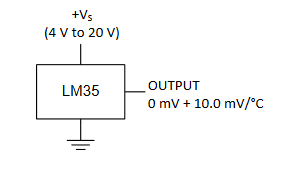
\includegraphics{LM35_config_basica}
			\caption{Diagrama do LM35 na configuração básica}
			\label{Rotulo}
		\end{figure}
		\subsection{Sensor de umidade do Solo Higrômetro}
		Sensor é capaz de perceber variações da umidade do solo, tem saída em volts que é linearmente depende da umidade.
		Trabalha com tensão de Operação: 3,3-5v, o que torna viável sua utilização com o Arduino. Tem saída digital em Led, com a sensibilidade calibrada por potenciômetro. Mas essa função não será utilizada no projeto.
	
		\subsection{Sensor de luminosidade LDR 5mm }
		
		Sensor de Luminosidade LDR de 5mm de diâmetro. Este sensor altera a resistência em seus terminais conforme a luminosidade a que é submetido.
		
		Especificações:
		Resistência quando há luz : ~1k Ohm.
		
		Resistência no escuro : ~10kOhm.
		
		Tensão máxima: 150V.
		
		Potência máxima: 100mW.
		
		\subsection{Plataforma arduino - Mega}	
		\subsection{Mecânica}
			Falar da bomba, da válvula solenóide, do controle das persianas.	
	
		
	\section{Projeto de software}
		
\chapter{Implementação}

\chapter{Conclusões}

 
 
\addcontentsline{toc}{chapter}{Bibliografia}
\bibliographystyle{coppe}
\bibliography{My_Collection_used}	
	
	
	
	
	
	
	
	
	
	
	
		
	
	
	

\end{document}          
